\documentclass{report}
 
\usepackage[utf8]{inputenc} 
\usepackage[T1]{fontenc}      
\usepackage[top=3.5cm, bottom=3cm, left=3.0cm, right=4.0cm]{geometry}
\usepackage{graphicx}
\usepackage{amsmath}
\graphicspath{{figures/}{../figures}}

\begin{document}

\chapter*{Oscillateurs quasi-sinusoïdaux, AO en régime linéaire et saturé - corrigé}

\newpage

\section*{Correction Exercice 1}

\begin{itemize}
	\item[•] 
	\begin{equation}
		i(t) + \left[(1-G)R_2C_1 +R_1C_1+R_2C_2\right]\frac{di(t)}{dt}+R_1C_1R_2C_2\frac{d^2i(t)}{dt^2}=0 
	\end{equation}
	\item[•]  $G=\frac{R_1C_1+R_2C_2+R_2C_1}{R_2C_1}$ et $f_0=\frac{1}{2\pi(R_1C_1R_2C_2)}$
	\item[•] On remplace $R_2\leftarrow\frac{R_2R_e}{R_2+R_e}$ et $R_1\leftarrow R_1+R_s$
\end{itemize}

\section*{Correction exercice 2}

\subsubsection{Amplificateur idéal}


\begin{itemize}
	\item[•] La boucle de rétroaction est sur la borne +, l'AO est en régime saturé et donc $u_s=\pm V_s$. 
	\item[•] Condition de basculement de $+/-V_s\rightarrow-/+V_s$ : $u_-\rightarrow-/+\frac{R_1}{R_2+R_1}$.
	On peut commencer par $u_-(t=0)=\frac{R_1}{R_2+R_1}V_s$ et $u_+(t=0)=-V_s$. Alors :
	\begin{equation}
		u_-(t)=V_s\left(1+\frac{R_1}{R_1+R_2}\right)\exp(-t/RC)-V_s 
	\end{equation}
Puis, à $t=t_1=RC\ln\left(\frac{2R_1+R_2}{R_2} \right)$ :
	\begin{equation}
		u_-(t)=-V_s\left(1+\frac{R_1}{R_1+R_2}\right)\exp(-(t-t_1)/RC)+V_s 
	\end{equation}
Et ainsi de suite. La période est donc $T = 2RC\ln\left(\frac{2R_1+R_2}{R_2} \right)$. $u_+(t)$ évolue en créneau de même période. 
\end{itemize}

\subsubsection{Amplificateur réel}

On trouve :

\begin{align*}
	\left\lbrace
\begin{array}{cc}
	& \tau_0\frac{du_s}{dt} +u_s = \mu_0(u_+-u_-) \\
	&  u_+=\frac{R_1+R_2}{R_1}\\
	&\tau_1\frac{du_-}{dt} +u_- =u_s  \\
\end{array}\right.
\end{align*}

On arrive alors sur deux équations différentielles couplées :
\begin{align*}
	\left\lbrace
\begin{array}{cc}
	& \tau_0\frac{du_s}{dt} = \mu_1u_s - \mu_0u_- \\
	&  \\
	&\tau_1\frac{du_-}{dt} = u_s - u_-  \\
\end{array}\right.
\end{align*}
avec $\mu_1=\mu_0\frac{R_1+R_2}{R_1}-1\simeq\mu_0\frac{R_1+R_2}{R_1}$.

On toruve alors une ED sur $u_s$ :
\begin{equation}
	\frac{d^2u_s}{dt^2} +\left( \frac{1}{\tau_1}-\frac{\mu_1}{\tau_0}\right) \frac{du_s}{dt} + \frac{1}{\tau_1\tau_0}\left(\mu_0-\mu_1\right)u_s=0
\end{equation}
Comme $\mu_0<\mu_1$, les solutions sont exponentielles et divergentes. On se retrouve donc très rapidement dans le régime d'instabilité même si les conditions initiales sont nulles (la moindre perturbatiosn étant amplifiée).
\section*{Correction exercice 3}

\begin{itemize}
	\item[•]
	\begin{equation}
		H=\frac{jRC\omega}{1+3jRC\omega-(RC\omega)^2}=\frac{1/3}{1+\frac{j}{3}\left( \frac{\omega}{\omega_0}-\frac{\omega_0}{\omega}\right) }
	\end{equation}
	donc $Q=1/3$ et $\omega_0=1/RC$.
	\item[•] Équation différentielle : $\omega_0\frac{du_e}{dt}=u_s+3\omega_0\frac{du_s}{dt}+\omega_0^2\frac{d^2u_s}{dt}$. Comme $u_s = (1+R_2/R_1)u_e$, on a :
	\begin{equation}
	0=u_s+\left( 2-\frac{R_2}{R_1}\right) \omega_0\frac{du_s}{dt}+\omega_0^2\frac{d^2u_s}{dt}
	\end{equation}
	Oscillations si $R_2=2R_1$.
	\item[•] Quasi-sinusoïdal car pour démarrer on a besoin de la condition $R_2>2R_1$ et alors solutions exponentielles divergentes, jusqu'à saturation. Le démarrage se fait à partir du bruit de fond qui est amplifié. 
\end{itemize}

\section*{Correction exercice 4}

\begin{itemize}
	\item[•] C'est un passe-bande d'ordre 2. Soit $u_1$ le potentiel entre la résistance $R$, la capacité $C$ et l'inductance $L_1$. Alors :
	\begin{equation}
		\frac{u_1}{u_e}=\frac{1}{1+R\left(\frac{1}{jL\omega}+ jC\omega \right) }
	\end{equation}
	De même :
	\begin{equation}
		\frac{u_s}{u_1}=\frac{jL_2\omega}{jL_1\omega+jL_2\omega}
	\end{equation}
	Alors : 
	\begin{equation}
		\frac{u_s}{u_e}=\frac{A_0}{1+jQ\left( \frac{\omega}{\omega_c}- \frac{\omega}{\omega_c}\right)}
	\end{equation}
	avec $\omega_c=\frac{1}{\sqrt{(L_1+L_2)C}}$, $A_0=\frac{L_2}{L_1+L_2}$ et $Q=RC\omega_c=R\sqrt{\frac{C}{L_1+L_2}}$
	
	\item[•] La fonction de transfert totale faite du filtre et de l'amplificateur d'écrit : 
		\begin{equation}
		\frac{u'_s}{u_e}=\frac{R_1+R_2}{R_1}\frac{A_0}{1+jQ\left( \frac{\omega}{\omega_0}- \frac{\omega}{\omega_0}\right)}=\frac{R_1+R_2}{R_1}\frac{A_0}{1+jR\left(C\omega- \frac{1}{L\omega}\right)}
	\end{equation}
	Le circuit est quasi-sinusoïdal s'il existe une pulsaiton $\omega_0$ tq $\mid F(j\omega_0)\mid=1$ et $arg\left[F(j\omega_0 \right] =0 $.
	
	On peut passer aussi par l'équation différentielle.
	On trouve $\omega_0=\omega_c$ et la condition :
	\begin{equation}
		\frac{R_1+R_2}{R_1}\frac{L_2}{L_1+L_2}=1
	\end{equation}
\end{itemize}

\subsubsection{Question supplémentaire}

On ne peut avoir des oscillations qu'avec un basse bande. Pour un filtre passe-haut et passe-bas, on ne peut avoir que des solutions divergentes ou qui tendent vers 0. On peut le trouver avec les fonctions canoniques.
	
\section*{Remplissage d'un réservoir d'hélium}

\subsection*{Première version}
\begin{itemize}
	\item[•] Pas de boucle de rétroaction : l'AO fonctionne forcément en régime saturé car la condition $u_+=u_-$ n'est jamais remplie. L'AO marche donc en comparateur et comme il est parfait $I_+=i_-=0$. Les résistances $R_1$ et $R_2$ sont inutiles.
	\item[•] Le potentiomètre fonctionne comme 2 résistances $(1-x)R_P$ et $xR_P$. Le potentiel (au niveau de la flèche) est pris entre ces 2 résistances. On a donc $u_+=\frac{xR_P+R_3}{R_P+R_3}U$, avec $U=5$V. La vanne s'ouvre lorsque $u_+>u_-$ cad pour :
	\begin{equation}
		u_+>u_-\Rightarrow\frac{xR_P+R_3}{R_P+R_3}U>\alpha h_{min}
	\end{equation}
	De même, la vanne se ferme lorsque :
	\begin{equation}
		u_+<	u_-\Rightarrow\frac{xR_P+R_3}{R_P+R_3}U<\alpha h_{max}
	\end{equation}
	On trouve que $h_{min}=h_{max}\in\left[ 0,2;1\right] $ pour x variant de 0 à 1.
	On a donc bien un système qui verse de l'hélium lorsque la hauteur descend en dessous de $h_{min}$ et s'arrête lorsque la hauteur atteint $h_{max}$. Le défaut est que $h_{min}=h_{max}$ : la vanne s'ouvre et se referme en permanence.
\end{itemize}

\subsection*{Seconde version}

\begin{itemize}
	\item[•] L'AO fonctionne toujours en régime saturé car la boucle de rétroaction est sur la borne +. $u_P$ est inchangé car les résistances $R_1$ sont très grandes devant les autres. On a donc $u_+=\frac{1}{2}u_s +\frac{1}{2}u_p$
	Si la vanne est initialement fermée, celle-ci s'ouvre lorsque le niveau atteint un niveau $h_{min}$ qui correspond à :
	\begin{equation}
		u_+=\frac{1}{2}V_{sat+} +\frac{1}{2}u_p=\alpha h_{min}
	\end{equation}
De même, si la vanne est initialement ouverte, celle-ci se ferme lorsque le niveau atteint un niveau $h_{max}$ qui correspond à :
	\begin{equation}
		u_+=\frac{1}{2}V_{sat-} +\frac{1}{2}u_p=\alpha h_{min}
	\end{equation}
	
	On a alors : $h_{min}=0,1$m et $h_{max}=1,1$m si $x=0$ et $h_{min}=0,5$m et $h_{max}=1,5$m si $x=1$. Le système ne s'ouvre et ferme plus en permanence.
\end{itemize}

\section*{Électrolyse du sulfate de Cobalt}

\subsubsection*{Quelques rappels}

Un réaction d'oxydo-réduction : $\alpha Ox + ne^-\longrightarrow \beta Red$.

Potentiel de Nernst : $E_N=E_0+\frac{0,06}{n}\log\frac{a_{ox}^\alpha}{a_{red}^\beta}$

Anode : $E_a>E_N$ siège de l'oxydation $\beta Red \longrightarrow \alpha Ox + ne^- $.
Cathode : $E_c<E_N$ siège de la réduction $\alpha Ox + ne^-\longrightarrow \beta Red$

\subsubsection*{Correction}

\begin{itemize}
	\item[•] Équation  bilan de cémentation : Fe + Cu$^{2+}\longrightarrow$ Cu + Fe$^{2+}$.
	Pour Co/Co$^{2+}$, $E_C\sim-0,29-0,15=-0,44$V donc la réaction Fe + Co$^{2+}\longrightarrow$ Co + Fe$^{2+}$ est thermodynamiquement possible mais cinétiquement bloquée. Seul Cu$^{2+}$ réagit avec Fe, le Cobalt reste en solution.
	\begin{figure}[!h]
	\centering
	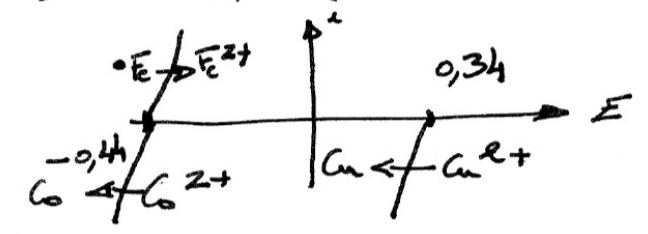
\includegraphics[width=0.5\linewidth]{Chimie1.png}
	\end{figure}

	\item[•] Les espèces présentes sont : H$_2$O, Co$^{2+}$ et SO$_{4}^{2-}$.
	
	A l'anode on peut avoir :  
	
	H$_2$O $\longrightarrow\frac{1}{2}$O$_2$ + 2H$^+$ + 2e$^-$, avec $E_N=1,23-0,06$pH=1,05V
	
	A la cathode, on peut avoir : 
	
	 Co$^{2+}$+ 2e$^-\longrightarrow$ Co, avec $E_N=-0.29+\frac{0.06}{2}\log[\mathrm{Co}^{2+}]$=-0,31V\footnote{La concentration en Co pour CoSO$_4$, 7H$_2$O à 50g.L$^{-1}$ est de 0.18mol/L comme $M=281$g/mol.}

	 2H$^{+}$+ 2e$^-\longrightarrow$ 2H, avec $E_N=-0,06$pH=-0,18V
	 
	 Sans surtension, on réalise l'électrolyse de l'eau avec $\Delta E_{min}=1,23$V.
	 
	 \item[•] $E_{A1} =$ 1,05+0,7=1,75V, $E_{C1} =$ -0,18+0,4=-0,58V et $E_{C2} =$ -0,41V
	 
	 Avec les surtensions, les potentiels à la cathode sont inversés. On réalise l'électrolyse du cobalt. 
	 \begin{figure}[!h]
	\centering
	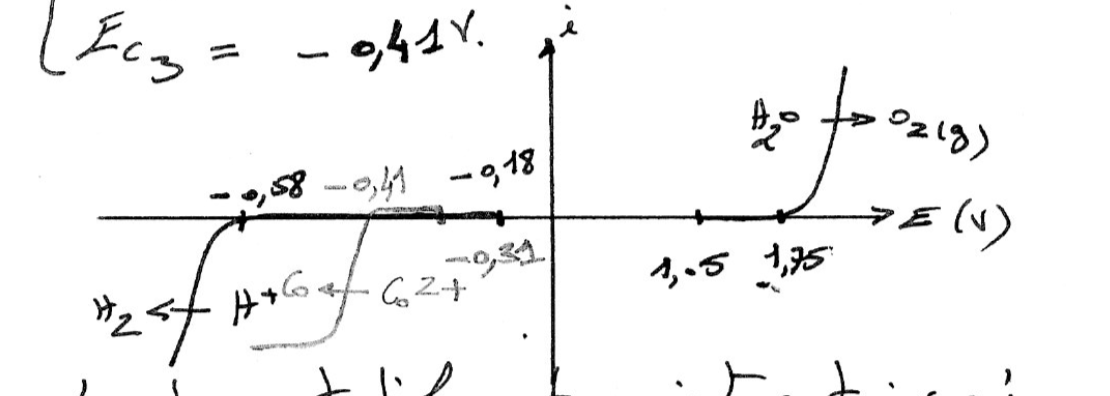
\includegraphics[width=0.8\linewidth]{Chimie2.png}
	\end{figure}

	 \item[•] L'électrolyse est sous contrôle cinétique, car on "repousse" la courbe de la réduction de $H^+$ avec une surtension, cad avec une considération cinétique : 
	 
	 Co$^{2+}$ + H$_2$O $\longrightarrow\frac{1}{2}$O$_2$ + 2H$^+$ + Co
	 \item[•] 
	 
	 On a : $\Delta E = E_{ohmique} + E_{N, O_2/H_2O} + \eta_{O_2/H_2O} - ( E_{N,Co/Co^{2+}} + \eta_{Co})$
	 
	$E_{N, O_2/H_2O}=1,23-0,06pH=1,05$V
	 
	 Il faut calculer $E_{N,Co/Co^{2+}}$ :
	 
	 $n$(SO$_{4}^{2-}$, 7H$_2$O) = $m$(SO$_{4}^{2-}$, 7H$_2$O)$M$(SO$_{4}^{2-}$, 7H$_2$O)=0,18 mol.
	 
	 Comme c'est la quantité pour 1L, [Co$^{2+}$]=0,18 mol.L$^{-1}$. Alors $E_{N,Co/Co^{2+}}=-0,29+0.03\log$[Co$^{2+}$]=-0.31V.
	 
	  A courant nul, $\Delta E_{min}=1,75-0,41$=2,16V, avec la chute ohmique $\Delta E_{min}=3,26$ V.
	  
	  \item[•] La charge échangée en un jour est : $C=I\Delta t$=8,64$\cdot$10$^8$C, cad une quantité de $C/F=8953$ moles d'électrons échangés. Comme pour deux électrons consommés, il n'ya qu'un Co qui est crée :
	  $n_{Co}=4477$ moles, cad 264kg de Co.
	  \item[•] $\eta=0,97$. Il y a toujours une petite quantité d'H$_2$ qui est formée, au détriment du Co, à cause de la faible différence entre les potentiels.
	  \item[•] On consomme $E= UI\Delta t$=3,02GJ. Il faut donc 11,8MJ pour créer 1kg de Co.
\end{itemize}

\end{document}
